\subsection{bsp e}

\[
  P_e=t^4(t+1)\partial_t^4 + t\partial_t^2+\frac{1}{t}\partial_t+1
\]

\begin{center}
  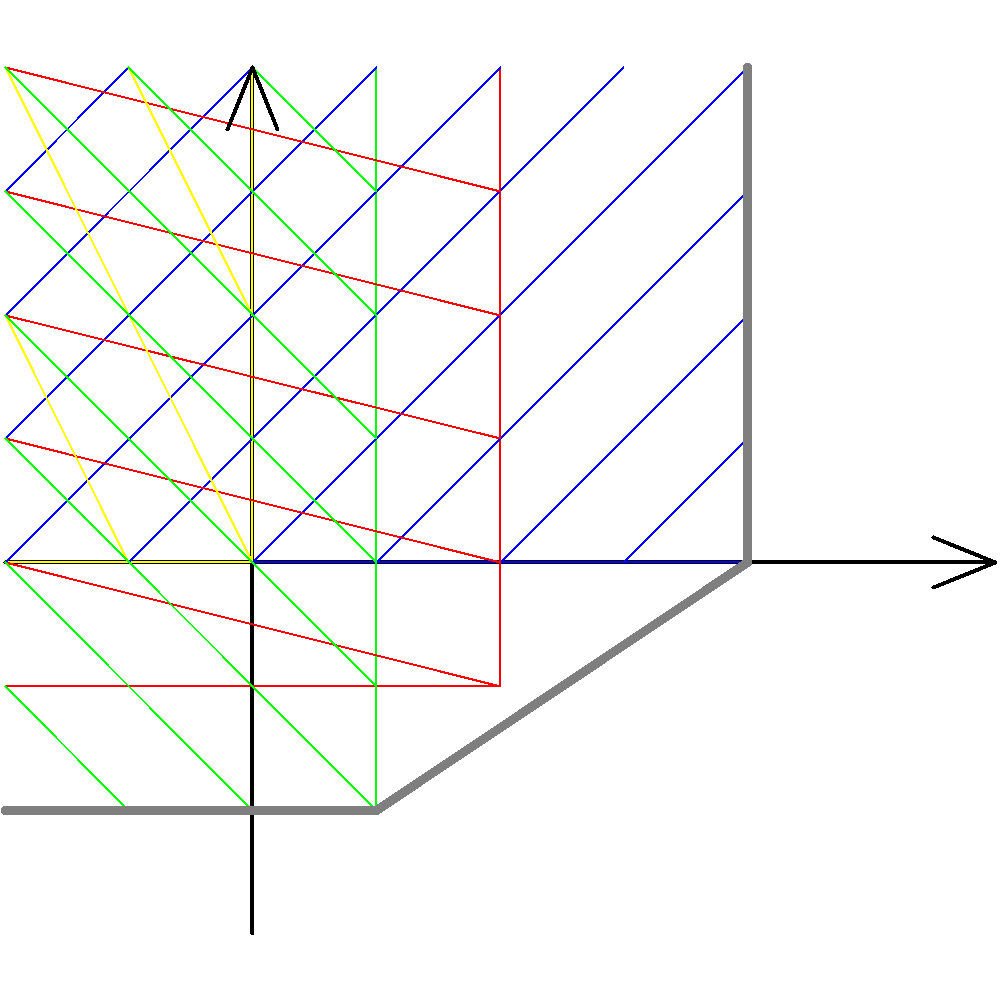
\includegraphics[width=6cm]{beispiele/img/e.png}
\end{center}

also $\slopes(P_e)=\{0,\frac{2}{3}\}$

Dies gilt Analog für das einfachere:
\[
  \bar P_e=t^4\partial_t^4 +\frac{1}{t}\partial_t
\]

\begin{center}
  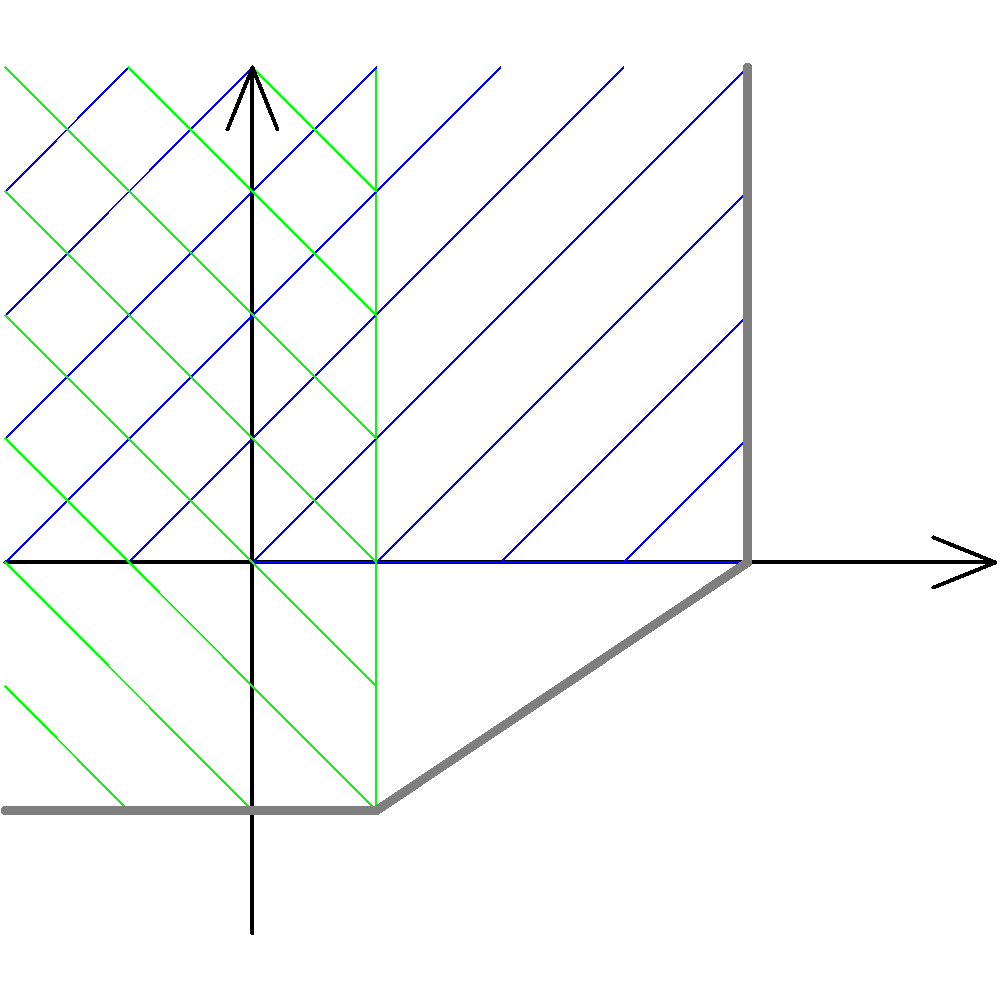
\includegraphics[width=6cm]{beispiele/img/bar_e.png}
\end{center}

% vim: set ft=tex :
